\documentclass[12pt, titlepage]{article}

\usepackage{fullpage}
\usepackage[round]{natbib}
\usepackage{multirow}
\usepackage{booktabs}
\usepackage{tabularx}
\usepackage{graphicx}
\usepackage{float}
\usepackage{hyperref}
% --- ADDED: Packages for color and strikethrough ---
\usepackage{color}
\usepackage[normalem]{ulem}
% --- END ADDED ---
\hypersetup{
    colorlinks,
    citecolor=blue,
    filecolor=black,
    linkcolor=red,
    urlcolor=blue
}

%% Comments

\usepackage{color}

\newif\ifcomments\commentstrue %displays comments
%\newif\ifcomments\commentsfalse %so that comments do not display

\ifcomments
\newcommand{\authornote}[3]{\textcolor{#1}{[#3 ---#2]}}
\newcommand{\todo}[1]{\textcolor{red}{[TODO: #1]}}
\else
\newcommand{\authornote}[3]{}
\newcommand{\todo}[1]{}
\fi

\newcommand{\wss}[1]{\authornote{blue}{SS}{#1}} 
\newcommand{\plt}[1]{\authornote{magenta}{TPLT}{#1}} %For explanation of the template
\newcommand{\an}[1]{\authornote{cyan}{Author}{#1}}

%% Common Parts

\newcommand{\progname}{ProgName} % PUT YOUR PROGRAM NAME HERE
\newcommand{\authname}{Team \#, Team Name
\\ Student 1 name
\\ Student 2 name
\\ Student 3 name
\\ Student 4 name} % AUTHOR NAMES                  

\usepackage{hyperref}
    \hypersetup{colorlinks=true, linkcolor=blue, citecolor=blue, filecolor=blue,
                urlcolor=blue, unicode=false}
    \urlstyle{same}
                                


\newcounter{acnum}
\newcommand{\actheacnum}{AC\theacnum}
\newcommand{\acref}[1]{AC\ref{#1}}

\newcounter{ucnum}
\newcommand{\uctheucnum}{UC\theucnum}
\newcommand{\uref}[1]{UC\ref{#1}}

\newcounter{mnum}
\newcommand{\mthemnum}{M\themnum}
\newcommand{\mref}[1]{M\ref{#1}}

\begin{document}

\title{Module Guide for \progname{}}
\author{\authname}
\date{\today}

\maketitle

\pagenumbering{roman}

\section{Revision History}

\begin{tabularx}{\textwidth}{p{3cm}p{2cm}X}
\toprule {\bf Date} & {\bf Version} & {\bf Notes}\\
\midrule
Date 1 & 1.0 & Notes\\
Date 2 & 1.1 & Notes\\
\bottomrule
\end{tabularx}

\newpage

\section{Reference Material}

This section records information for easy reference.

\subsection{Abbreviations and Acronyms}

\renewcommand{\arraystretch}{1.2}
\begin{tabular}{l l}
  \toprule
  \textbf{symbol} & \textbf{description}\\
  \midrule
  AC & Anticipated Change\\
  DAG & Directed Acyclic Graph \\
  M & Module \\
  MG & Module Guide \\
  OS & Operating System \\
  R & Requirement\\
  SC & Scientific Computing \\
  SRS & Software Requirements Specification\\
  \progname & Explanation of program name\\
  UC & Unlikely Change \\
  \textcolor{red}{HH} & \textcolor{red}{Hardware-Hiding} \\
  \textcolor{red}{BH} & \textcolor{red}{Behaviour-Hiding} \\
  \textcolor{red}{SD} & \textcolor{red}{Software Decision} \\
  \textcolor{red}{DB} & \textcolor{red}{Database} \\
  \textcolor{red}{GUI} & \textcolor{red}{Graphical User Interface} \\
  \textcolor{red}{CI/CD} & \textcolor{red}{Continuous Integration / Continuous Deployment} \\
  \wss{etc.} & \wss{...}\\
  \bottomrule
\end{tabular}\\

\newpage

\tableofcontents

\listoftables

\listoffigures

\newpage

\pagenumbering{arabic}

\section{Introduction}

Decomposing a system into modules is a commonly accepted approach to developing
software.  A module is a work assignment for a programmer or programming
team~\citep{ParnasEtAl1984}.  We advocate a decomposition
based on the principle of information hiding~\citep{Parnas1972a}.  This
principle supports design for change, because the ``secrets'' that each module
hides represent likely future changes.  Design for change is valuable in SC,
where modifications are frequent, especially during initial development as the
solution space is explored.

Our design follows the principles laid out by \citet{ParnasEtAl1984}, as follows:
\begin{itemize}
    \item System details that are likely to change independently are the secrets of separate modules.
    \item Each data structure is implemented in only one module, ensuring clarity and responsibility for managing that structure.
    \item Any program requiring information from a module's data structures must access it via well-defined interfaces.
\end{itemize}

The MES-ERP financial platform's design focuses on:
\begin{itemize}
    \item Modularity: Each functional requirement is encapsulated in a distinct module to isolate changes and enhance maintainability.
    \item Scalability: Modules are designed to accommodate future enhancements, such as support for new input formats or integration with third-party systems.
    \item Robustness: Validation and error-handling mechanisms ensure data integrity across all modules.
\end{itemize}

After completing the Software Requirements Specification (SRS), the Module Guide (MG) was developed~\citep{ParnasEtAl1984}. The MG specifies the modular structure of the system and is intended to allow both designers and maintainers to easily identify and work on the system's components.

The potential readers of this document include:
\begin{itemize}
    \item New Project Members: Provides an overview of the system's structure, allowing new members to quickly identify relevant modules.
    \item Maintainers: Ensures maintainers can understand and update the system while minimizing the impact on unrelated modules.
    \item Designers: Allows designers to verify consistency, feasibility, and flexibility of the system's architecture.
\end{itemize}

\section{Anticipated and Unlikely Changes} \label{SecChange}

This section lists possible changes to the system, categorized as either anticipated or unlikely. These changes reflect both user-driven requirements and system-level constraints.

\subsection{Anticipated Changes} \label{SecAchange}

Anticipated changes are those expected to occur due to user feedback, evolving requirements, or regular system updates. These changes are addressed by hiding information in the appropriate modules.

\begin{description}
\item[\refstepcounter{acnum} \actheacnum \label{acInput}:] Input Data Format
\begin{itemize}
    \item \textcolor{red}{Secret:} \textcolor{red}{The specific format (e.g., CSV, JSON, potentially OCR from images) of receipt/expense data.}
    \item Impacted Modules: \sout{Input Format Module, Data Validation Module} \textcolor{red}{Expense Submission Module, Data Validation Module}
    \item Examples: Adding support for new formats (e.g., images, PDFs) or OCR for scanned receipts.
\end{itemize}

\item[\refstepcounter{acnum} \actheacnum \label{acNotifications}:] Notification Methods
\begin{itemize}
    \item \textcolor{red}{Secret:} \textcolor{red}{The specific method (Email, SMS, In-App) and external service (SendGrid, Twilio) used for notifications.}
    \item Impacted Modules: Notification System \textcolor{red}{Module}
    \item Examples: Adding SMS or push notification support.
\end{itemize}

\item[\refstepcounter{acnum} \actheacnum \label{acWorkflow}:] Reimbursement Workflow \textcolor{red}{Rules}
\begin{itemize}
    \item \textcolor{red}{Secret:} \textcolor{red}{The specific rules defining the steps, conditions, and approvers for processing requests.}
    \item Impacted Modules: \sout{Reimbursement Submission, Approval Workflow} \textcolor{red}{Approval Workflow Module}
    \item Examples: Modifying approval rules \textcolor{red}{(e.g., adding budget holder sign-off)}, changing thresholds, or automating \sout{incomplete submission rejections} \textcolor{red}{rejection for incomplete submissions}.
\end{itemize}

\item[\refstepcounter{acnum} \actheacnum \label{acReporting}:] \textcolor{red}{Financial Reporting Formats}
\begin{itemize}
    \item \textcolor{red}{Secret:} \textcolor{red}{The specific format (PDF, CSV, Excel) and content structure of generated financial reports.}
    \item \textcolor{red}{Impacted Modules:} \textcolor{red}{Reporting Module}
    \item \textcolor{red}{Examples:} \textcolor{red}{Adding new report types (e.g., budget variance), changing export formats.}
\end{itemize}
\end{description}

\subsection{Unlikely Changes} \label{SecUchange}

Unlikely changes are less probable due to their disruptive nature or misalignment with project goals.

\begin{description}
\item[\refstepcounter{ucnum} \uctheucnum \label{ucTechStack}:] \textcolor{red}{Core} Technology Stack
\begin{itemize}
    \item Impacted Modules: All
    \item Examples: Switching from TypeScript/Next.js to another framework \textcolor{red}{(e.g., Python/Django, Java/Spring)}.
\end{itemize}

\item[\refstepcounter{ucnum} \uctheucnum \label{ucDatabase}:] \textcolor{red}{Database Provider}
\begin{itemize}
    \item \textcolor{red}{Impacted Modules:} \textcolor{red}{Database Interaction Layer Module}
    \item \textcolor{red}{Examples:} \textcolor{red}{Migrating from Supabase/PostgreSQL to MySQL, MongoDB, or a self-hosted solution.}
\end{itemize}
\end{description}

\section{Module Hierarchy} \label{SecMH}

Modules are organized to encapsulate secrets and ensure clear responsibilities. The hierarchy reflects relationships between modules and their dependencies, as shown in Table \ref{TblMH}. \textcolor{red}{This decomposition follows the standard Hardware-Hiding (HH), Behaviour-Hiding (BH), and Software Decision (SD) layers.}

\begin{description}
\item [\refstepcounter{mnum} \mthemnum \label{mHH}:]
\textbf{Hardware-Hiding Module\textcolor{red}{s}:} Abstracts \sout{database and file system} \textcolor{red}{interactions with external hardware or services, primarily the database}.
\item [\refstepcounter{mnum} \mthemnum \label{mBH}:]
\textbf{Behaviour-Hiding Module\textcolor{red}{s}:} Implements \sout{workflows for submissions, reviews, and dashboards} \textcolor{red}{the externally visible functionality specified in the SRS}.
\item [\refstepcounter{mnum} \mthemnum \label{mSD}:]
\textbf{Software Decision Module\textcolor{red}{s}:} Encapsulates \sout{shared logic for validation, testing, and CI/CD} \textcolor{red}{internal design choices, algorithms, or data structures not directly visible to the user but necessary for implementation}.
\end{description}

\begin{table}[H]
\centering
\renewcommand{\arraystretch}{1.5}
\begin{tabular}{p{0.3\textwidth} p{0.6\textwidth}}
\toprule
\textbf{Level 1} & \textbf{Level 2}\\
\midrule
\textcolor{red}{Hardware-Hiding (HH)} & \textcolor{red}{Database Interaction Layer (\mref{mDB})} \\
\midrule
\multirow{8}{0.3\textwidth}{\textcolor{red}{Behaviour-Hiding (BH)}}
& \textcolor{red}{User Authentication \& Profile Management (\mref{mUserAuth})} \\ 
& \textcolor{red}{Expense Submission \& Tracking (\mref{mExpenseSub})} \\ 
& \textcolor{red}{Budget and Funding Management (\mref{mBudgetMgmt})} \\ 
& \textcolor{red}{Approval Workflow and Review (\mref{mApproval})} \\ 
& \textcolor{red}{Notifications \& Communication (\mref{mNotify})} \\ 
& \textcolor{red}{Policy \& Compliance Management (\mref{mCompliance})} \\ 
& \textcolor{red}{Reporting and Analytics (\mref{mReporting})} \\ 
& \textcolor{red}{Administrator and Configuration Panel (\mref{mAdminPanel})} \\ 
\midrule
\multirow{2}{0.3\textwidth}{\textcolor{red}{Software Decision (SD)}} 
& \textcolor{red}{Data Validation Module (\mref{mValidation})} \\
& \textcolor{red}{GUI Module (\mref{mGUI})} \\

\bottomrule
\end{tabular}
\caption{Module Hierarchy}
\label{TblMH}
\end{table}


\section{Connection Between Requirements and Design}

The design of the MES-ERP system has been structured to ensure that the requirements outlined in the Software Requirements Specification (SRS) are met comprehensively. Table~\ref{tab:req-to-modules} illustrates the connection between the requirements and the modules designed to fulfill them.

\begin{table}[h!]
\centering
\caption{Connection Between Requirements and Modules}
\label{tab:req-to-modules}

\begin{tabular}{|p{4cm}|p{8cm}|}
\hline
\textbf{Requirement (R)} & \textbf{Modules} \\
\hline
R1: Secure Authentication & \textcolor{red}{User Authentication \& Profile Management Module (\mref{mUserAuth})} \\
\hline
R2: Expense Submission \& Tracking & \textcolor{red}{Expense Submission \& Tracking Module (\mref{mExpenseSub})} \\
\hline
R3: Budget Validation & \textcolor{red}{Budget and Funding Management Module (\mref{mBudgetMgmt})} \\
\hline
R4: Approval Workflow & \textcolor{red}{Approval Workflow and Review Module (\mref{mApproval})} \\
\hline
R5: Notifications & \textcolor{red}{Notifications \& Communication Module (\mref{mNotify})} \\
\hline
R6: Compliance & \textcolor{red}{Policy \& Compliance Management Module (\mref{mCompliance})} \\
\hline
R7: Reporting & \textcolor{red}{Reporting and Analytics Module (\mref{mReporting})} \\
\hline
R8: Administrative Tools & \textcolor{red}{Administrator and Configuration Panel Module (\mref{mAdminPanel})} \\
\hline
\end{tabular}
\end{table}

\subsection{Design Decisions for Each Requirement}

\begin{itemize}
    \item \textbf{R1: Secure Authentication}
    \begin{itemize}
        \item \textbf{Module}: \textcolor{red}{User Authentication \& Profile Management Module (\mref{mUserAuth})}
        \item \textbf{Design Decision}: Implements secure login \textcolor{red}{via Supabase Auth}, \sout{with} session timeouts, role-based access control \textcolor{red}{(RBAC)}, and \sout{account lockout mechanisms} \textcolor{red}{profile management}.
    \end{itemize}

    \item \textbf{R2: Expense Submission \& Tracking}
    \begin{itemize}
        \item \textbf{Module}: \textcolor{red}{Expense Submission \& Tracking Module (\mref{mExpenseSub})}
        \item \textbf{Design Decision}: Provides forms for submission, receipt uploads (\textcolor{red}{incl. OCR attempt}), and tracking expense status \textcolor{red}{via the database}.
    \end{itemize}

    \item \textbf{R3: Budget Validation}
    \begin{itemize}
        \item \textbf{Module}: \textcolor{red}{Budget and Funding Management Module (\mref{mBudgetMgmt})}
        \item \textbf{Design Decision}: Ensures expense requests \sout{do not exceed departmental budgets} \textcolor{red}{are checked against allocated group budgets} and integrates with \sout{the financial system} \textcolor{red}{the operating budget data stored in the database}.
    \end{itemize}

    \item \textbf{R4: Approval Workflow}
    \begin{itemize}
        \item \textbf{Module}: \textcolor{red}{Approval Workflow and Review Module (\mref{mApproval})}
        \item \textbf{Design Decision}: Implements dynamic routing for approvals \textcolor{red}{(based on role/group)} and \sout{notifications for pending actions} \textcolor{red}{triggers status updates}.
    \end{itemize}

    \item \textbf{R5: Notifications}
    \begin{itemize}
        \item \textbf{Module}: \textcolor{red}{Notifications \& Communication Module (\mref{mNotify})}
        \item \textbf{Design Decision}: Sends alerts via email\sout{, SMS,} and \sout{dashboard notifications} \textcolor{red}{(using SendGrid)} for \sout{system events} \textcolor{red}{request status changes}. \textcolor{red}{(SMS is a potential future extension)}.
    \end{itemize}

    \item \textbf{R6: Compliance}
    \begin{itemize}
        \item \textbf{Module}: \textcolor{red}{Policy \& Compliance Management Module (\mref{mCompliance})}
        \item \textbf{Design Decision}: Validates expense requests against predefined policies \textcolor{red}{(e.g., spending limits, required documentation)} \sout{to ensure compliance with regulations}. \textcolor{red}{Includes audit logging of key actions.}
    \end{itemize}

    \item \textbf{R7: Reporting}
    \begin{itemize}
        \item \textbf{Module}: \textcolor{red}{Reporting and Analytics Module (\mref{mReporting})}
        \item \textbf{Design Decision}: Generates \sout{detailed reports in PDF/CSV format} \textcolor{red}{on-screen analytics visualizations (charts/tables)} for expense tracking and system usage. \textcolor{red}{(Export functionality (PDF/CSV) is an anticipated change \acref{acReporting})}.
    \end{itemize}

    \item \textbf{R8: Administrative Tools}
    \begin{itemize}
        \item \textbf{Module}: \textcolor{red}{Administrator and Configuration Panel Module (\mref{mAdminPanel})}
        \item \textbf{Design Decision}: Enables administrators to manage user roles, \sout{configure approval workflows,} \textcolor{red}{groups, permissions,} and access \sout{system logs} \textcolor{red}{the operating budget interface}.
    \end{itemize}
\end{itemize}

\section{Module Decomposition} \label{SecMD}

The MES-ERP system is designed following the principle of \textit{information hiding}, which ensures that each module encapsulates decisions likely to change independently. The modules are organized into a hierarchy, with higher-level modules relying on lower-level ones for functionality. This hierarchy forms a directed acyclic graph (DAG). \sout{Figure~\ref{fig:module-decomposition} illustrates the module decomposition.} \textcolor{red}{Figure~\ref{fig:diagram} (in Section~\ref{SecUse}) illustrates the use relation between modules. The primary decomposition follows the HH, BH, and SD layers.} \textcolor{red}{Supporting processes like CI/CD and test automation, while crucial for development, are not considered core architectural modules in this decomposition as they do not hide specific design decisions related to the system's runtime behavior.}

\subsection{\textcolor{red}{Hardware-Hiding (HH) Modules}}

\begin{description}
\item[\refstepcounter{mnum} \mthemnum \label{mDB} \textbf{Database Interaction Layer:}]
    \begin{itemize}
        \item \textbf{Secrets:} The specific database technology (\textcolor{red}{Supabase/PostgreSQL}), schema details, query language (\textcolor{red}{SQL}), and connection management.
        \item \textbf{Services:} Provides abstract functions for creating, reading, updating, and deleting (CRUD) data related to users, groups, roles, requests, budgets, etc. Hides the underlying implementation details of data persistence.
        \item \textbf{Implemented By:} \textcolor{red}{Backend API using Supabase client library.}
    \end{itemize}
\end{description}

\subsection{\textcolor{red}{Behaviour-Hiding (BH) Modules}}

\begin{description}
\item[\refstepcounter{mnum} \mthemnum \label{mUserAuth} \textbf{User Authentication \& Profile Management:}]
    \begin{itemize}
        \item \textbf{Secrets:} The mechanism for verifying user identity (\textcolor{red}{delegated to Supabase Auth}), session management details, and the structure of user profile data (excluding role/group assignments handled elsewhere).
        \item \textbf{Services:} Provides functions for user login, registration, logout, retrieving profile information (\sout{name, email, etc.}), and updating profile details. \textcolor{red}{Corresponds to SRS R1.}
        \item \textbf{Implemented By:} \textcolor{red}{Backend API (using Supabase Auth), Frontend UI (Login/Register/Account Pages).}
    \end{itemize}

\item[\refstepcounter{mnum} \mthemnum \label{mExpenseSub} \textbf{Expense Submission \& Tracking:}]
    \begin{itemize}
        \item \textbf{Secrets:} The specific fields required for a request, receipt data format (\acref{acInput}) including OCR processing logic, and how request statuses are represented internally before approval.
        \item \textbf{Services:} Allows users to create new payment/reimbursement requests, upload receipts, view the status of their own submitted requests. \textcolor{red}{Corresponds to SRS R2.}
        \item \textbf{Implemented By:} \textcolor{red}{Frontend UI (Forms Page), Backend API (Request Creation Endpoint).}
    \end{itemize}

\item[\refstepcounter{mnum} \mthemnum \label{mBudgetMgmt} \textbf{Budget and Funding Management:}]
    \begin{itemize}
        \item \textbf{Secrets:} How budget allocations are stored and retrieved for groups, the rules for checking available funds against requests.
        \item \textbf{Services:} Provides functions to check if a request amount is within a group's allocated budget, potentially update remaining budget upon approval/reimbursement. Allows admins to view/manage operating budget lines. \textcolor{red}{Corresponds to SRS R3.}
        \item \textbf{Implemented By:} \textcolor{red}{Backend API (Budget Checking Logic), Frontend UI (Operating Budget Page).}
    \end{itemize}

\item[\refstepcounter{mnum} \mthemnum \label{mApproval} \textbf{Approval Workflow and Review:}]
    \begin{itemize}
        \item \textbf{Secrets:} The specific sequence of approval steps, the conditions for routing requests (\acref{acWorkflow}), and the internal representation of approval states.
        \item \textbf{Services:} Enables authorized users (admins) to view pending requests, change their status (approve/reject), and potentially add comments. Triggers notifications upon status change. \textcolor{red}{Corresponds to SRS R4.}
        \item \textbf{Implemented By:} \textcolor{red}{Backend API (Status Update Logic), Frontend UI (Requests Page for Admins).}
    \end{itemize}

\item[\refstepcounter{mnum} \mthemnum \label{mNotify} \textbf{Notifications \& Communication:}]
    \begin{itemize}
        \item \textbf{Secrets:} The specific notification channels (Email, \sout{SMS}) and the external services used (\acref{acNotifications}). The content templates for different notification types.
        \item \textbf{Services:} Provides a function to send notifications to users based on system events (e.g., request status change). \textcolor{red}{Corresponds to SRS R5.}
        \item \textbf{Implemented By:} \textcolor{red}{Backend API (Notification Endpoints using SendGrid).}
    \end{itemize}

\item[\refstepcounter{mnum} \mthemnum \label{mCompliance} \textbf{Policy \& Compliance Management:}]
    \begin{itemize}
        \item \textbf{Secrets:} The specific compliance rules checked during submission or approval (e.g., maximum request amounts, required fields based on type). The structure and storage of audit logs.
        \item \textbf{Services:} Validates requests against defined policies. Records significant actions (creation, update, deletion of requests/users/roles) in an audit log. \textcolor{red}{Corresponds to SRS R6.}
        \item \textbf{Implemented By:} \textcolor{red}{Backend API (Validation Logic, Audit Logging Hooks).}
    \end{itemize}

\item[\refstepcounter{mnum} \mthemnum \label{mReporting} \textbf{Reporting and Analytics:}]
    \begin{itemize}
        \item \textbf{Secrets:} The specific data aggregation methods and calculations used to generate analytics insights. The format of generated reports (\acref{acReporting}).
        \item \textbf{Services:} Provides aggregated data for display in analytics charts/tables (e.g., spending trends, status summaries). \textcolor{red}{Corresponds to SRS R7.}
        \item \textbf{Implemented By:} \textcolor{red}{Backend API (Analytics Data Endpoint), Frontend UI (Analytics Page with Charts).}
    \end{itemize}

\item[\refstepcounter{mnum} \mthemnum \label{mAdminPanel} \textbf{Administrator and Configuration Panel:}]
    \begin{itemize}
        \item \textbf{Secrets:} The specific administrative functions available (user management, role management, group management, budget configuration) and how configurations are stored.
        \item \textbf{Services:} Provides interfaces for administrators to manage core system entities like users, roles, groups, and the operating budget structure. \textcolor{red}{Corresponds to SRS R8.}
        \item \textbf{Implemented By:} \textcolor{red}{Frontend UI (Users, Roles, Groups, Operating Budget pages), Backend API (Endpoints for managing these entities).}
    \end{itemize}

\end{description}

\subsection{\textcolor{red}{Software Decision (SD) Modules}}

\begin{description}
\item[\refstepcounter{mnum} \mthemnum \label{mValidation} \textbf{Data Validation Module:}]
    \begin{itemize}
        \item \textbf{Secrets:} The specific validation rules (e.g., regex for emails, numeric checks for amounts, file type restrictions) and libraries used for input validation.
        \item \textbf{Services:} Provides functions to validate data submitted through forms or API requests, ensuring data consistency and integrity before it reaches the database or core logic modules.
        \item \textbf{Implemented By:} \textcolor{red}{Shared utility functions/library used by Backend API and potentially Frontend.}
    \end{itemize}

\item[\refstepcounter{mnum} \mthemnum \label{mGUI} \textbf{GUI Module:}]
    \begin{itemize}
        \item \textbf{Secrets:} The specific UI library (\textcolor{red}{Shadcn/ui}), CSS framework (\textcolor{red}{Tailwind}), and rendering engine (\textcolor{red}{React/Next.js}) used to build the user interface. The component structure and state management approach within the frontend.
        \item \textbf{Services:} Renders the web interface, handles user input events (clicks, form submissions), displays data fetched from the backend API, and manages frontend application state.
        \item \textbf{Implemented By:} \textcolor{red}{The entire Next.js frontend application code (\texttt{src/app}, \texttt{src/components}).}
    \end{itemize}
\end{description}

\section{Traceability Matrix}

This section outlines the anticipated changes \textcolor{red}{(from Section~\ref{SecAchange})} to the MES-ERP system and identifies the modules \textcolor{red}{(from Section~\ref{SecMD})} that would be impacted by each change. The traceability matrix maps these anticipated changes to the affected modules, ensuring alignment with the principle of \textit{information hiding}.

\subsection{Anticipated Changes to Modules}

Table~\ref{tab:anticipated-changes} provides a traceability matrix that lists the anticipated changes and their associated modules.

% --- REVISED Table 3 to use new module names and anticipated changes ---
\begin{table}[h!]
\centering
\caption{Traceability Matrix: Anticipated Changes to Modules}
\label{tab:anticipated-changes}
\begin{tabular}{|p{6cm}|p{8cm}|}
\hline
\textbf{Anticipated Change (AC)} & \textbf{Affected Modules} \\
\hline
\acref{acInput}: Input Data Format & \mref{mExpenseSub}, \mref{mValidation} \\ % AC1
\hline
\acref{acNotifications}: Notification Methods & \mref{mNotify} \\ % AC2
\hline
\acref{acWorkflow}: Reimbursement Workflow Rules & \mref{mApproval} \\ % AC3
\hline
\textcolor{red}{\acref{acReporting}: Financial Reporting Formats} & \textcolor{red}{\mref{mReporting}} \\ % AC4 (was AC7)
\hline
% Removed old AC1-AC8 as they were redundant/less specific
\end{tabular}
\end{table}

\subsection{Impact of Anticipated Changes}

% --- REVISED to discuss impact on new modules/secrets ---
\begin{itemize}
    \item \textbf{\acref{acInput}: Input Data Format}
    \begin{itemize}
        \item \textbf{Affected Modules}: \mref{mExpenseSub}, \mref{mValidation}
        \item \textbf{Impact}: \mref{mExpenseSub} would need updated logic for parsing new formats (e.g., adding OCR library call, handling XML). \mref{mValidation} would require new rules to check the validity of the new formats.
        \item \textbf{Mitigation}: Encapsulation of parsing logic within \mref{mExpenseSub} and validation rules within \mref{mValidation} isolates the impact.
    \end{itemize}

    \item \textbf{\acref{acNotifications}: Notification Methods}
    \begin{itemize}
        \item \textbf{Affected Module}: \mref{mNotify}
        \item \textbf{Impact}: Adding SMS would require integrating a new service (e.g., Twilio) within \mref{mNotify} and potentially adding phone numbers to user profiles (\mref{mUserAuth}).
        \item \textbf{Mitigation}: The abstract `sendNotification` service provided by \mref{mNotify} hides the specific channel implementation (Email vs. SMS) from calling modules like \mref{mApproval}.
    \end{itemize}

    \item \textbf{\acref{acWorkflow}: Reimbursement Workflow Rules}
    \begin{itemize}
        \item \textbf{Affected Module}: \mref{mApproval}
        \item \textbf{Impact}: Modifying approval steps (e.g., adding a second approver for amounts > \$1000) requires changing the internal state machine or rule engine within \mref{mApproval}.
        \item \textbf{Mitigation}: The workflow logic is contained within \mref{mApproval}, preventing changes from affecting submission (\mref{mExpenseSub}) or notification (\mref{mNotify}) modules directly.
    \end{itemize}

    \item \textbf{\textcolor{red}{\acref{acReporting}: Financial Reporting Formats}}
    \begin{itemize}
        \item \textbf{\textcolor{red}{Affected Module:}} \textcolor{red}{\mref{mReporting}}
        \item \textbf{\textcolor{red}{Impact:}} \textcolor{red}{Adding CSV export would require new data formatting logic and potentially a new function within \mref{mReporting}. Changing PDF layout involves modifying the PDF generation template/code used by this module.}
        \item \textbf{\textcolor{red}{Mitigation:}} \textcolor{red}{Report generation is isolated in \mref{mReporting}. Other modules only provide data to it, they don't depend on the output format.}
    \end{itemize}
\end{itemize}


\section{Use Hierarchy Between Modules} \label{SecUse}

In this section, the uses hierarchy between modules is
provided. \citet{Parnas1978} said of two programs A and B that A {\em uses} B if
correct execution of B may be necessary for A to complete the task described in
its specification. That is, A {\em uses} B if there exist situations in which
the correct functioning of A depends upon the availability of a correct
implementation of B. Figure \ref{FigUH} illustrates the use relation between
the modules. It can be seen that the graph is a directed acyclic graph
(DAG). Each level of the hierarchy offers a testable and usable subset of the
system, and modules in the higher level of the hierarchy are essentially simpler
because they use modules from the lower levels.

% --- Assume fig:diagram (Figure 1) will be updated by user to reflect new modules ---
\begin{figure}[H]
  \centering
  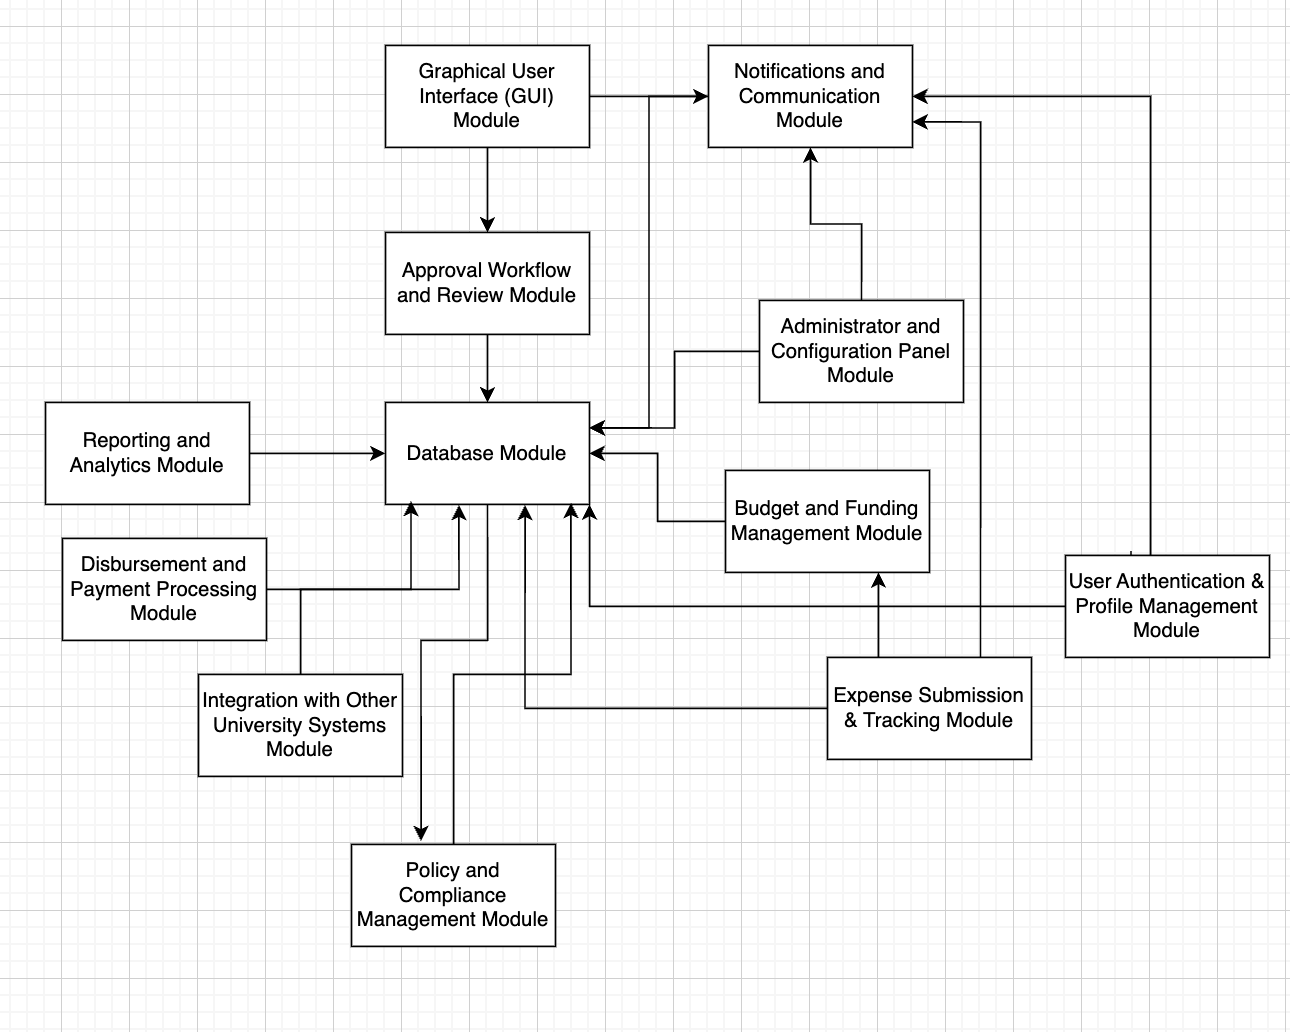
\includegraphics[width=1\textwidth]{img/diagram.png} % KEEPING FILENAME, assuming user updates the image file
  \caption{Module Use Hierarchy \textcolor{red}{(Illustrative - Requires Update based on Section~\ref{SecMD} modules)}} % Added note
  \label{fig:diagram} % Kept old label for consistency, might rename label AND \ref below if needed
  \label{FigUH} % Added this label as it was referenced in text above
\end{figure}

% --- ADDED: Textual description of uses relationships based on new modules ---
\textcolor{red}{
The dependencies shown in Figure~\ref{fig:diagram} (and implied by the decomposition) include:
\begin{itemize}
    \item Most Behaviour-Hiding (BH) and Software Decision (SD) modules \textbf{use} the \textbf{Database Interaction Layer (\mref{mDB})} to persist and retrieve data.
    \item The \textbf{GUI Module (\mref{mGUI})} \textbf{uses} many BH modules to display data and trigger actions, for example:
        \begin{itemize}
            \item Uses \textbf{User Authentication (\mref{mUserAuth})} for login/registration UI.
            \item Uses \textbf{Expense Submission (\mref{mExpenseSub})} to render forms and display request status.
            \item Uses \textbf{Budget Management (\mref{mBudgetMgmt})} to show budget dashboards.
            \item Uses \textbf{Approval Workflow (\mref{mApproval})} to display pending requests for admins.
            \item Uses \textbf{Reporting (\mref{mReporting})} to display analytics charts.
            \item Uses \textbf{Admin Panel (\mref{mAdminPanel})} to render user/role/group management interfaces.
        \end{itemize}
    \item The \textbf{Approval Workflow Module (\mref{mApproval})} \textbf{uses}:
        \begin{itemize}
            \item \textbf{Budget Management (\mref{mBudgetMgmt})} to check funds before approval.
            \item \textbf{Notifications (\mref{mNotify})} to send alerts after status changes.
            \item \textbf{Policy \& Compliance (\mref{mCompliance})} to log the approval action.
        \end{itemize}
    \item The \textbf{Expense Submission Module (\mref{mExpenseSub})} \textbf{uses}:
        \begin{itemize}
             \item \textbf{Data Validation (\mref{mValidation})} to check inputs before saving.
             \item \textbf{Policy \& Compliance (\mref{mCompliance})} to log the submission action.
        \end{itemize}
    \item The \textbf{Admin Panel (\mref{mAdminPanel})} \textbf{uses} modules like \textbf{User Authentication (\mref{mUserAuth})} (to manage user details), \textbf{Budget Management (\mref{mBudgetMgmt})} (to configure budgets), etc.
\end{itemize}
This structure aims for low coupling, where higher-level modules depend on the services provided by lower-level ones without knowing their internal implementation details.
}


% --- User Interfaces Section ---
% Added brief descriptions tying UIs to modules
\section{User Interfaces}

\subsection{Dashboard (\textcolor{red}{GUI Module - \mref{mGUI}})}
\begin{figure}[H]
    \centering
    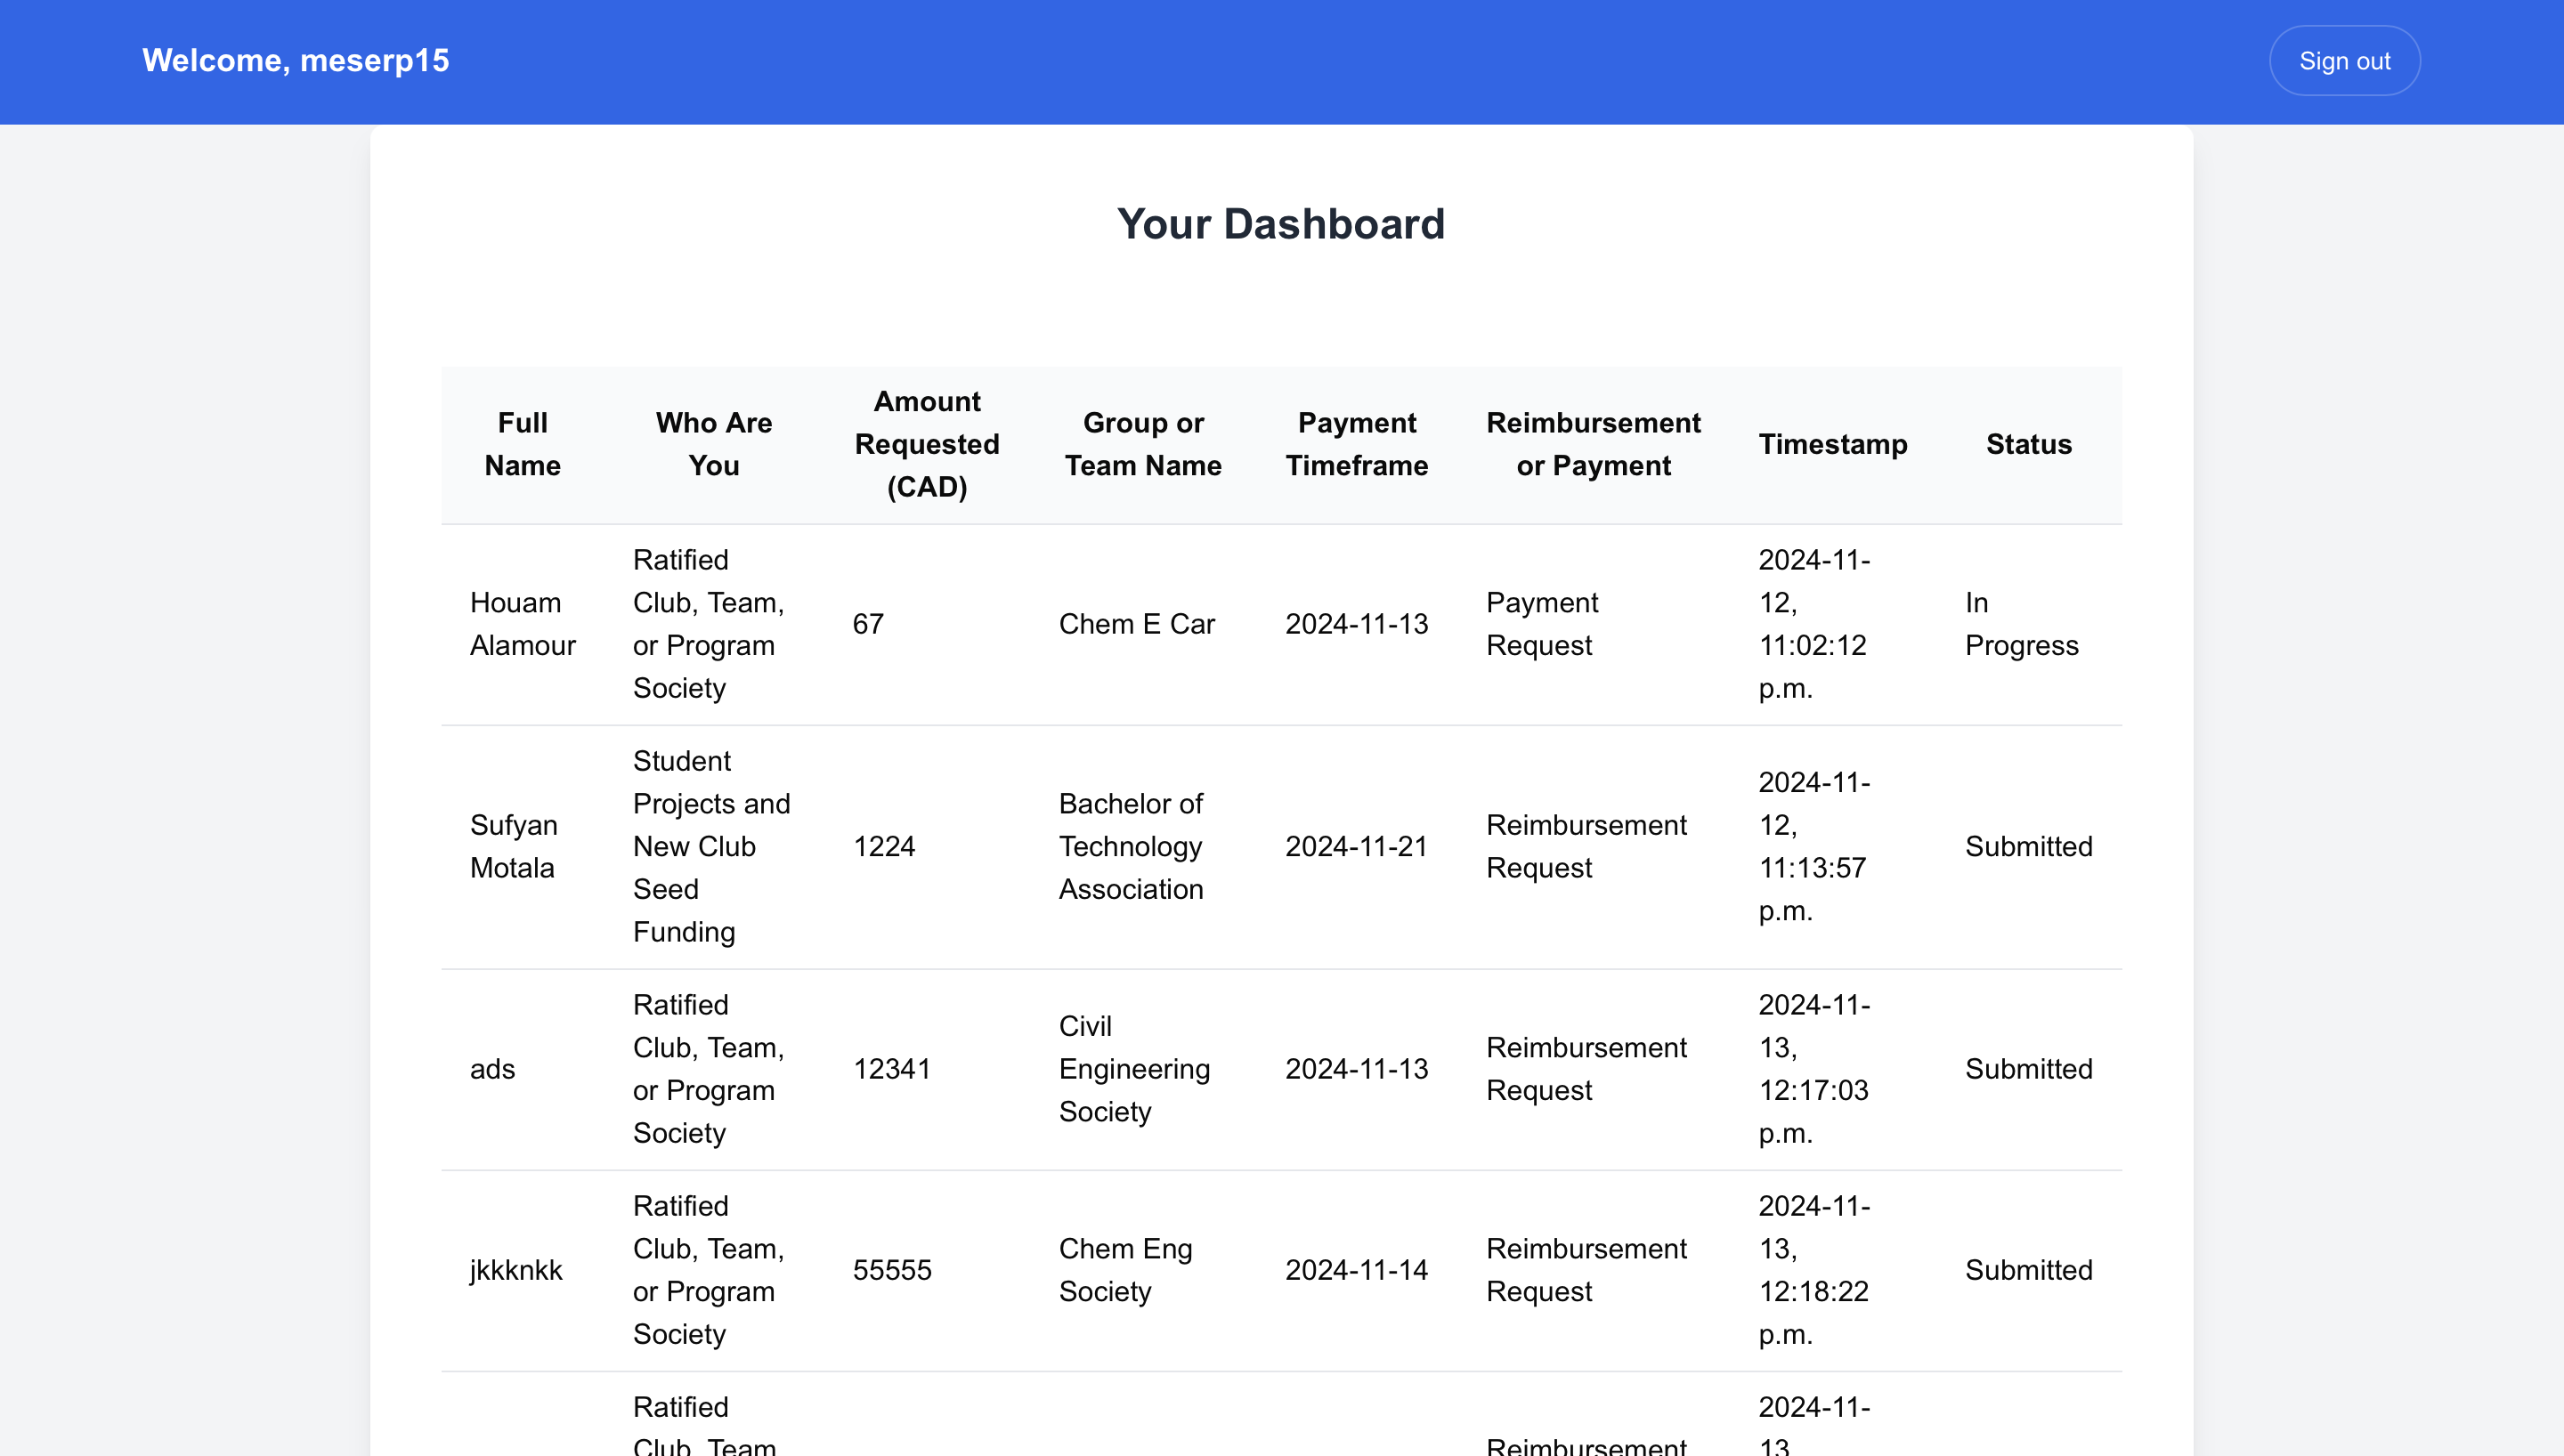
\includegraphics[width=0.8\textwidth]{img/dashboard.png}
    \caption{Dashboard View (\textcolor{red}{Presents data from \mref{mReporting}, \mref{mExpenseSub}})}
    \label{fig:dashboard}
\end{figure}

\subsection{Form (\textcolor{red}{GUI Module - \mref{mGUI}, uses \mref{mExpenseSub}})}
\begin{figure}[H]
    \centering
    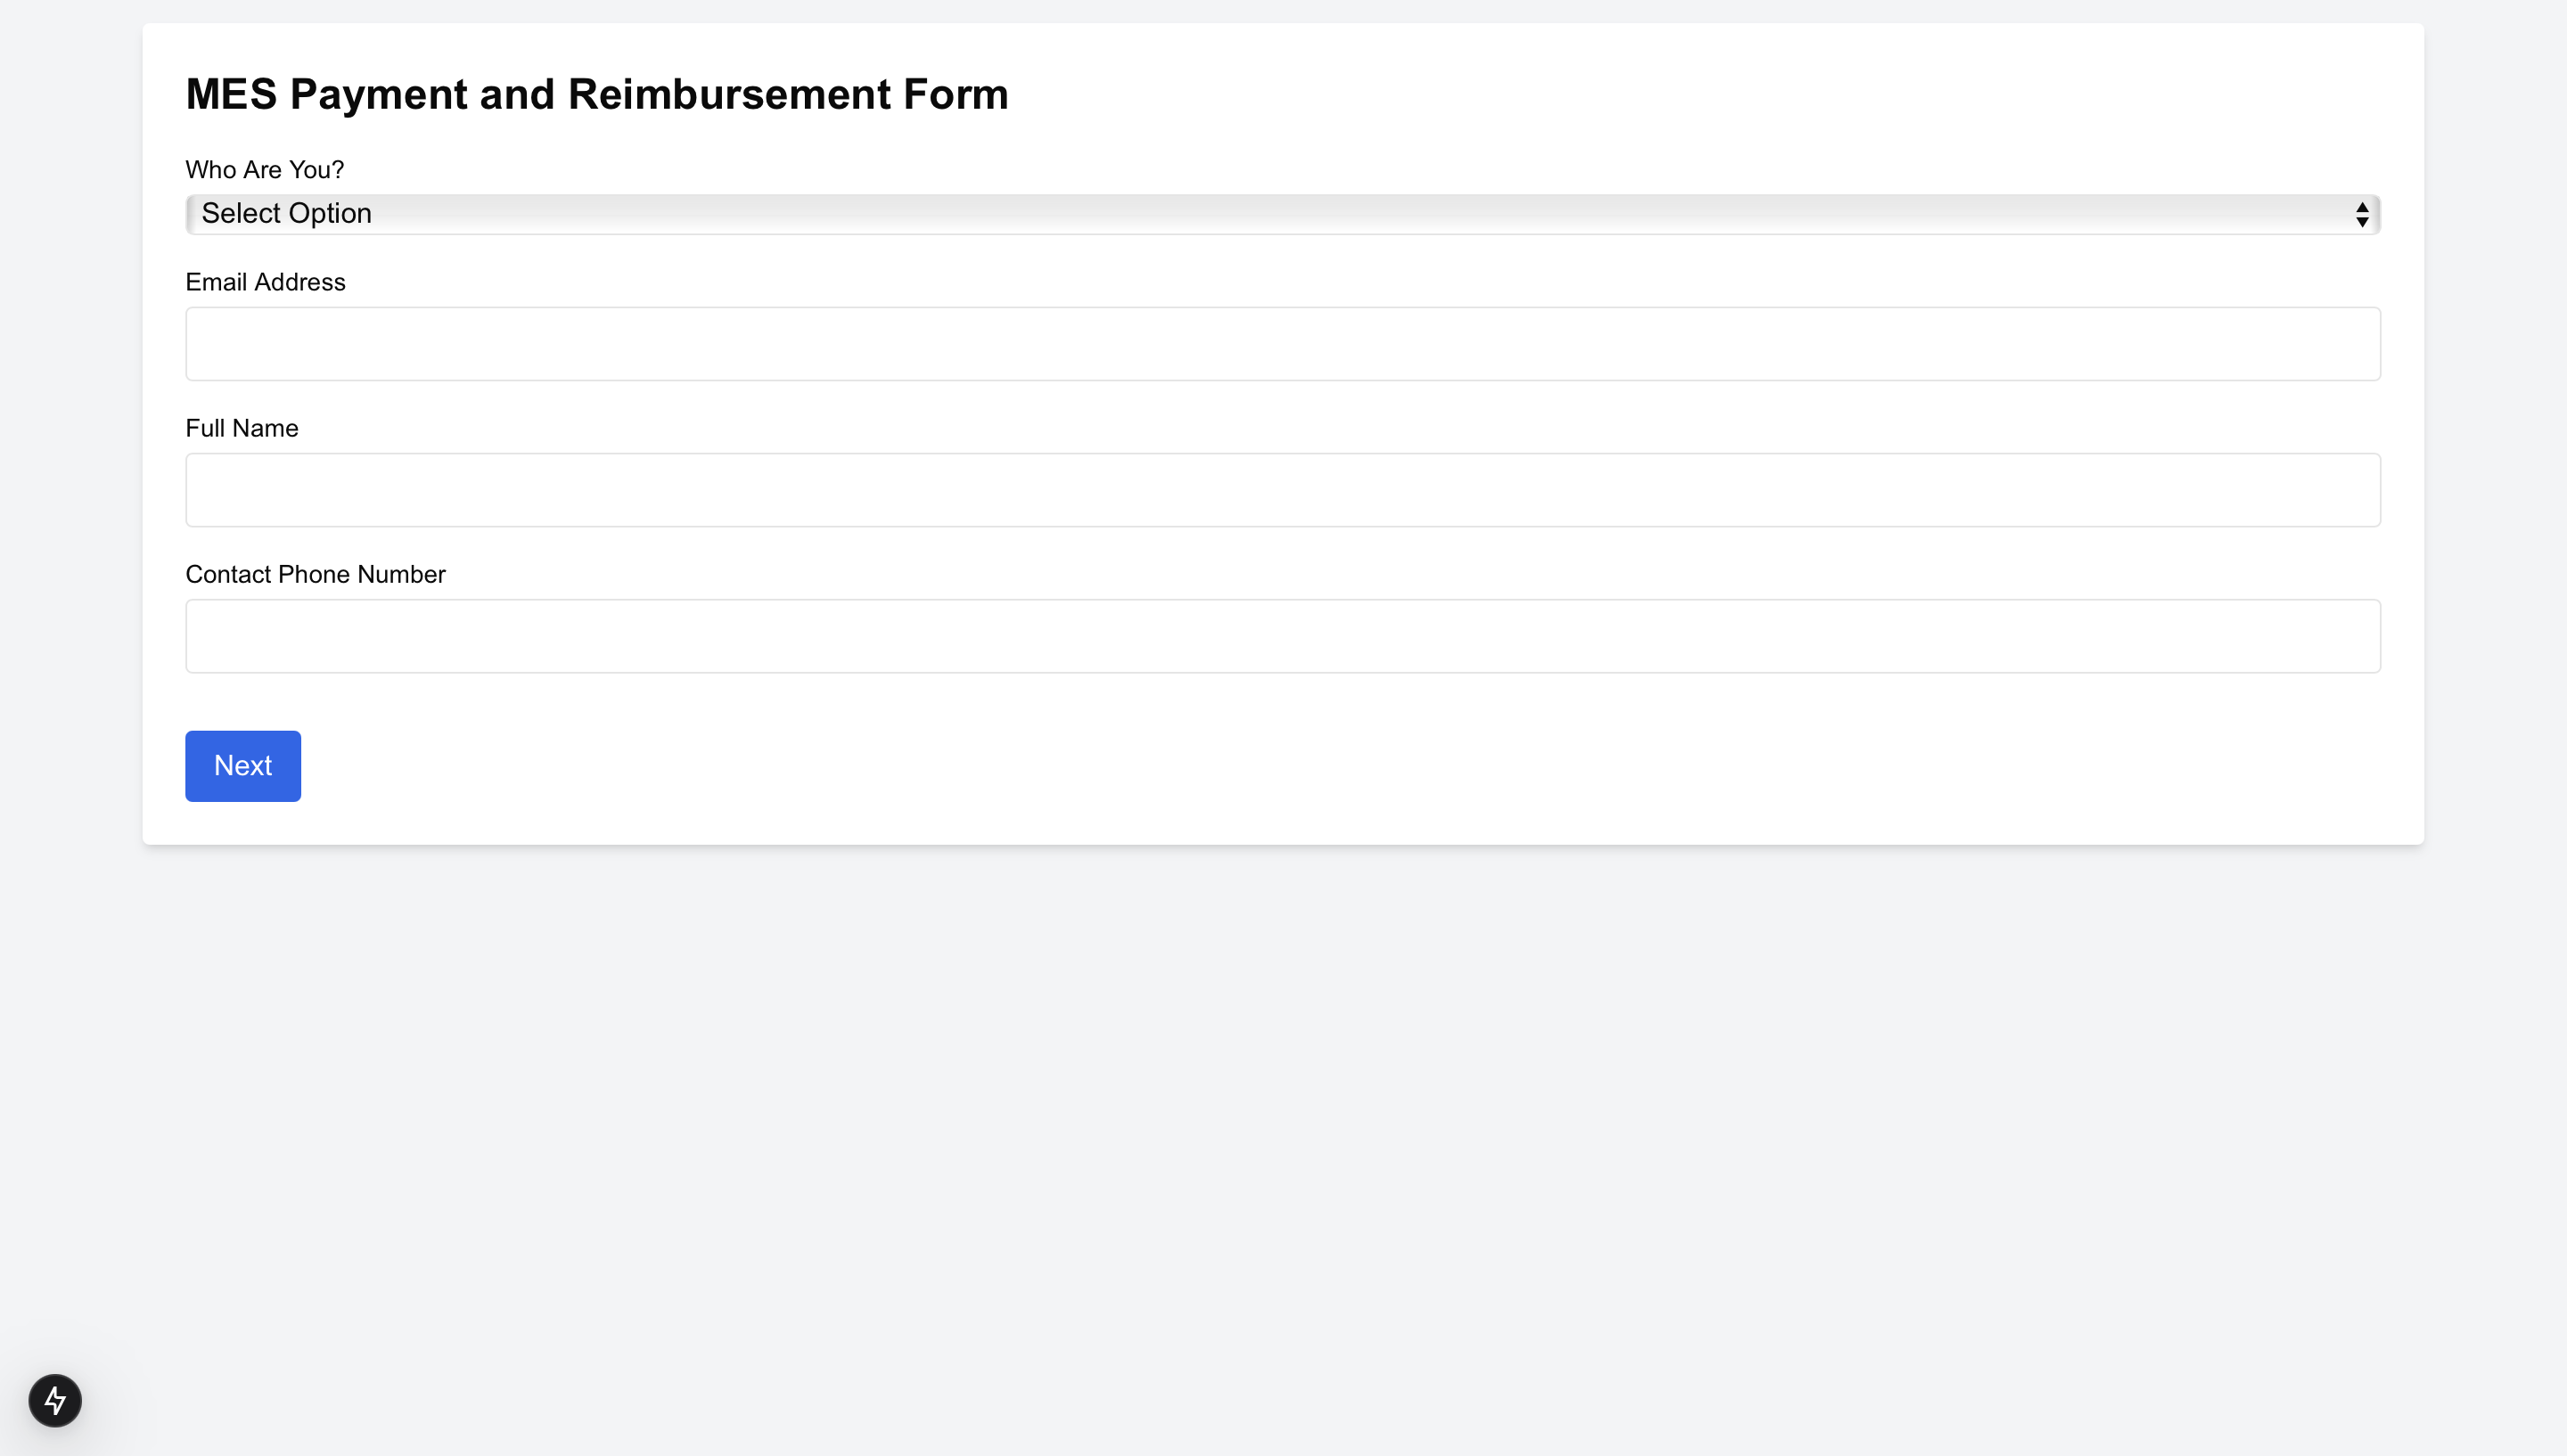
\includegraphics[width=0.8\textwidth]{img/form.png}
    \caption{Form View (\textcolor{red}{Interface for \mref{mExpenseSub}})}
    \label{fig:form}
\end{figure}

\subsection{Login (\textcolor{red}{GUI Module - \mref{mGUI}, uses \mref{mUserAuth}})}
\begin{figure}[H]
    \centering
    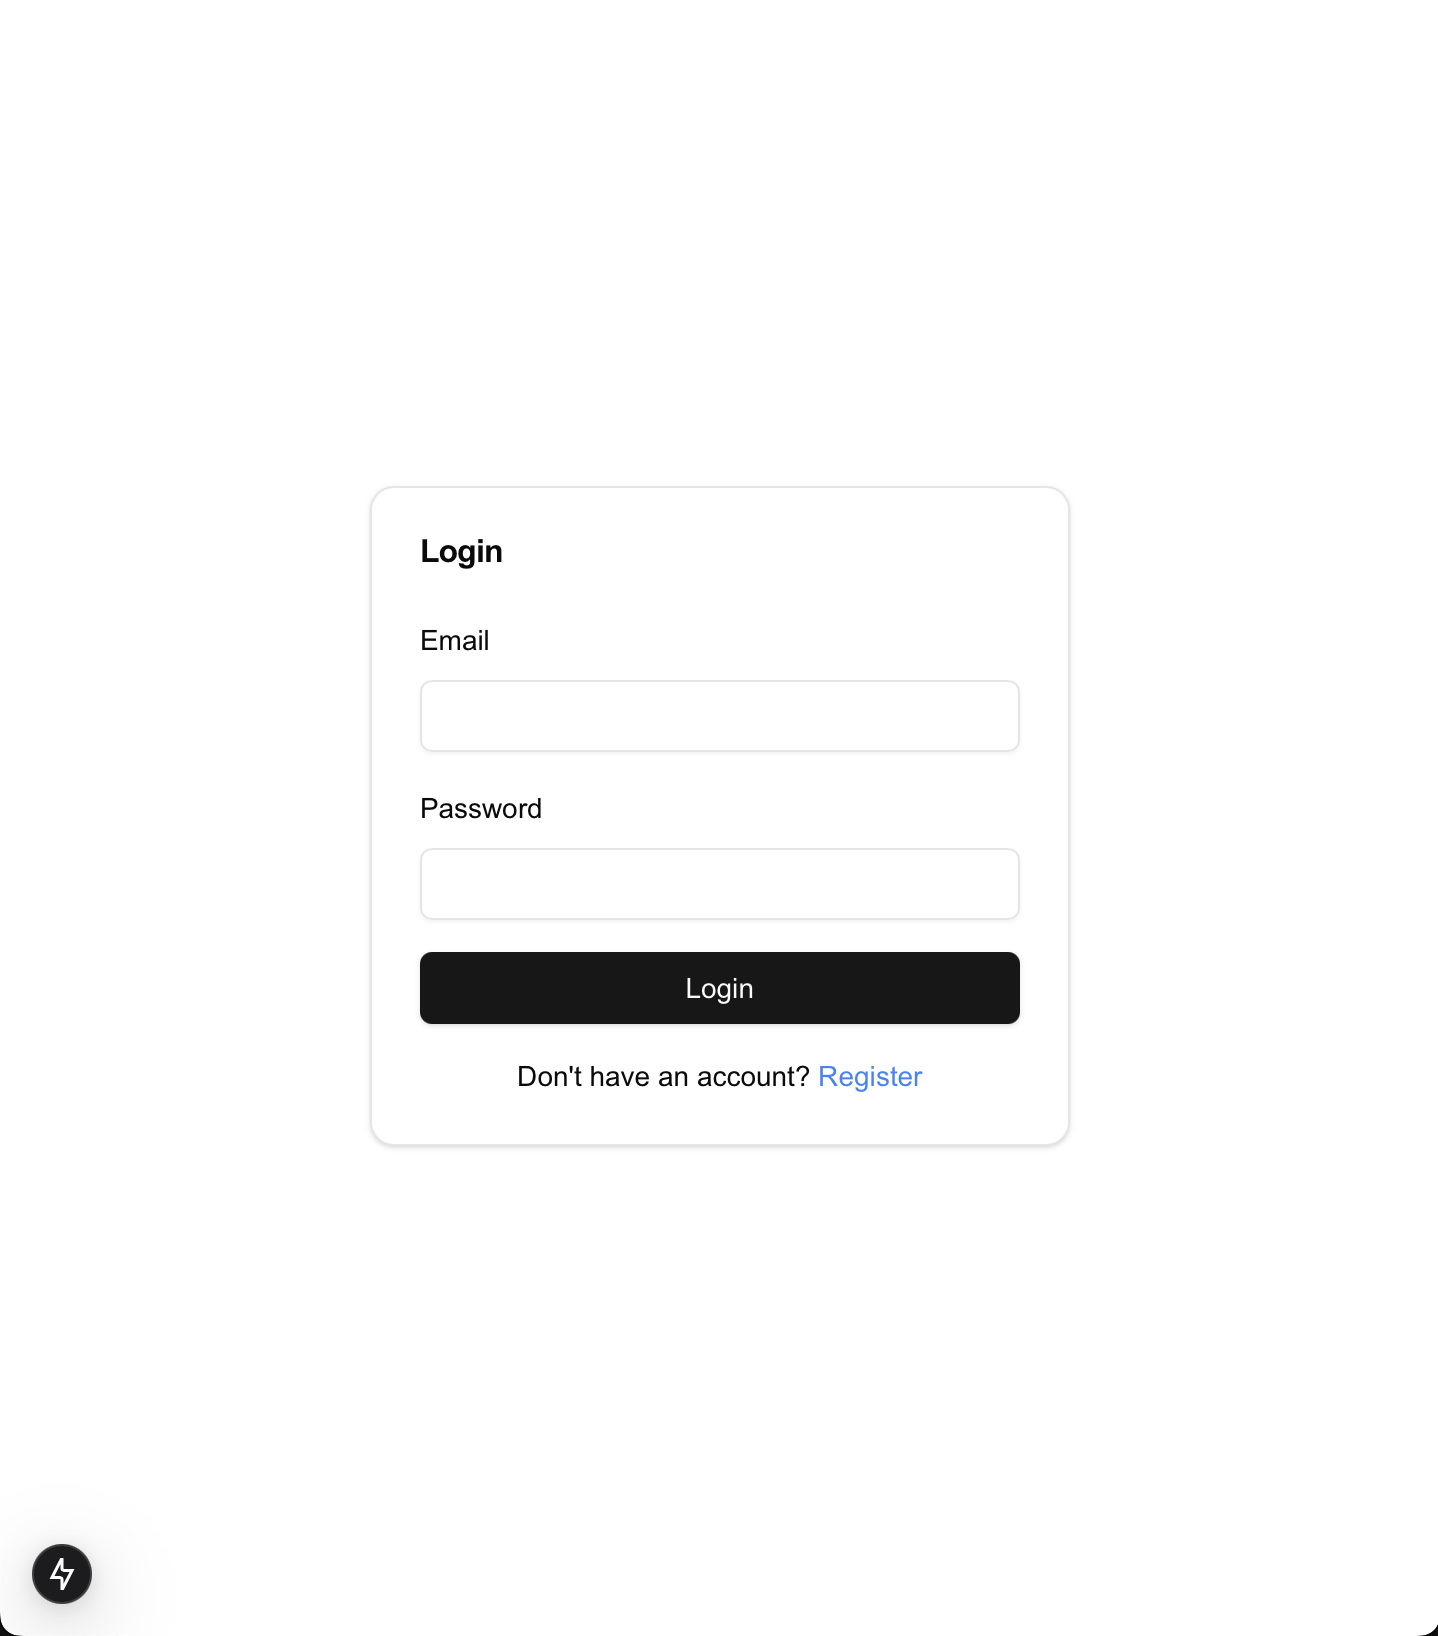
\includegraphics[width=0.8\textwidth]{img/login.png}
    \caption{Login View (\textcolor{red}{Interface for \mref{mUserAuth}})}
    \label{fig:login}
\end{figure}

\subsection{Receipt Input (\textcolor{red}{GUI Module - \mref{mGUI}, part of \mref{mExpenseSub}})}
\begin{figure}[H]
    \centering
    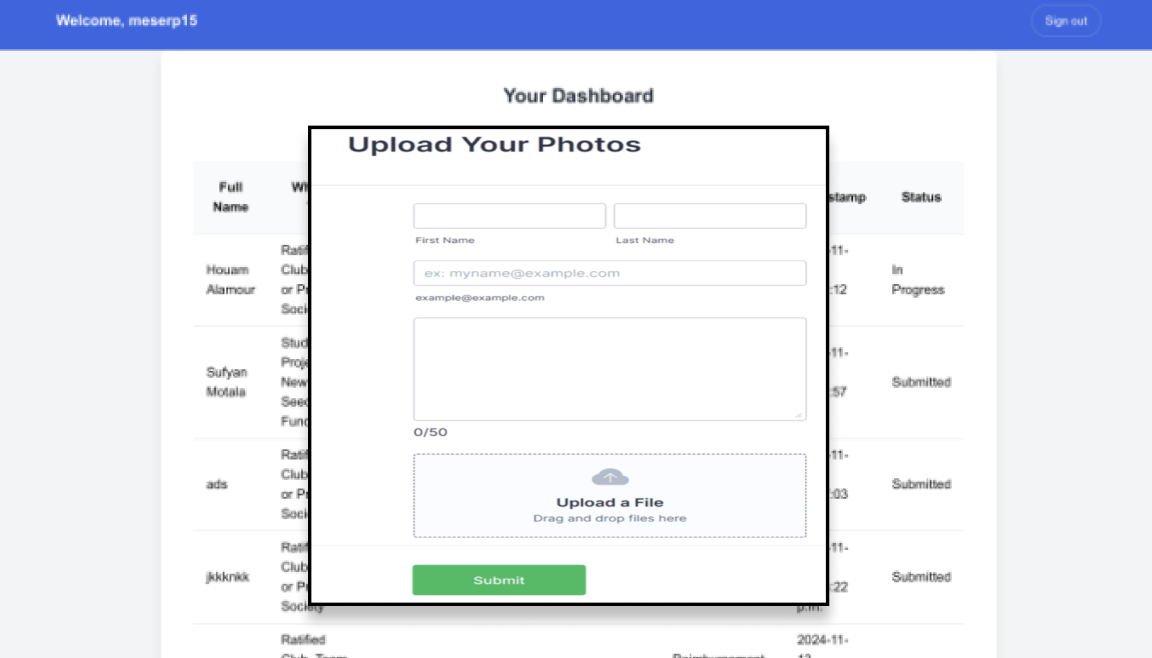
\includegraphics[width=0.8\textwidth]{img/upload.png}
    \caption{Receipt Scanning View (\textcolor{red}{Input for \mref{mExpenseSub}})}
    \label{fig:receipt}
\end{figure}

\subsection{Website Tutorial (\textcolor{red}{GUI Module - \mref{mGUI}})}
\begin{figure}[H]
    \centering
    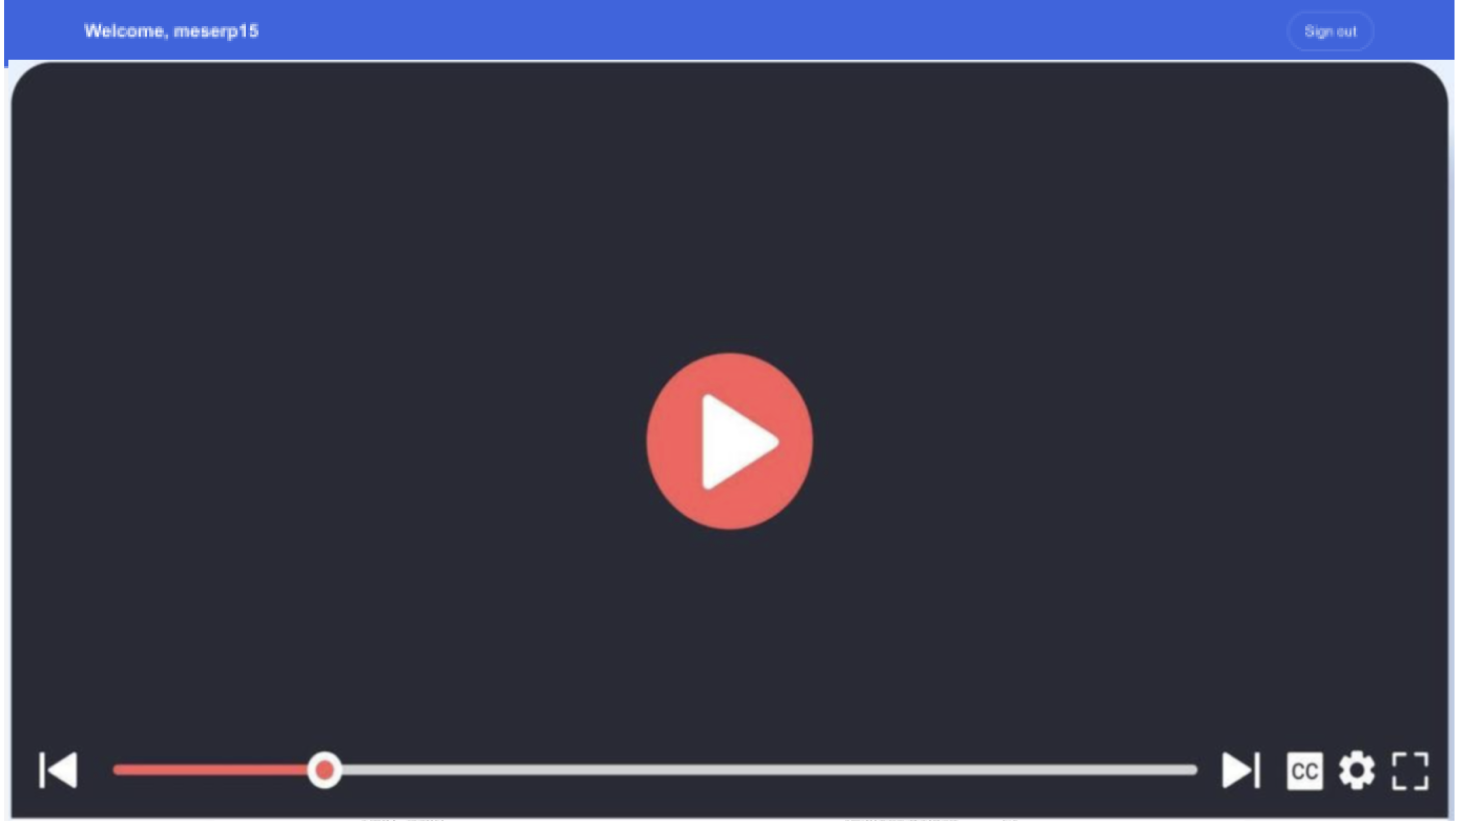
\includegraphics[width=0.8\textwidth]{img/tutorial.png}
    \caption{Tutorial Page}
    \label{fig:tutorial}
\end{figure}

% --- Design of Communication Protocols ---
% Clarified which modules handle these
\section{Design of Communication Protocols}

\begin{itemize}
  \item \textbf{APIs:} \textcolor{red}{The \textbf{GUI Module (\mref{mGUI})} uses} APIs \textcolor{red}{(implemented as Next.js API Routes)} to communicate between the backend and the frontend of the application.
  \item \textbf{Email Registration:} When creating an account\textcolor{red}{, the \textbf{User Authentication Module (\mref{mUserAuth})} (via Supabase Auth)} \sout{there} will \sout{be email authentication} \textcolor{red}{trigger email verification} to ensure valid users.
  \item \textbf{Email communication:} When a reimbursement request is \sout{made or} edited \textcolor{red}{or its status changes, the \textbf{Notifications Module (\mref{mNotify})}} \sout{, the correct groups} will \sout{be notified via email} \textcolor{red}{notify the relevant user via email}.
\end{itemize}

% --- Timeline Section ---
% Updated module names/references in the timeline descriptions
\section{Timeline}

\begin{itemize}
  \item \textbf{Team Formed, Project Selected:} September 16
  \begin{itemize}
    \item \textbf{All Team Members (Omar, Taaha, Rachid, Sufyan, Housam):}
    Establish initial roles, select project scope, and identify stakeholder needs.
  \end{itemize}

  \item \textbf{Problem Statement, POC Plan, Development Plan:} September 23
  \begin{itemize}
    \item \textbf{All Team Members:}
    Finalize the problem statement for the MES-ERP system. Outline Proof-of-Concept (POC) objectives and develop a high-level development plan.
    \item \textbf{Sufyan \& Omar:} Draft initial architecture sketches for key modules (\textcolor{red}{HH: \mref{mDB}}; \textcolor{red}{BH: e.g., \mref{mExpenseSub}}; \textcolor{red}{SD: e.g., \mref{mValidation}}).
  \end{itemize}

  \item \textbf{Requirements Document Revision 0:} October 9
  \begin{itemize}
    \item \textbf{Housam \& Rachid:} Gather and refine user stories for \textcolor{red}{Expense Submission (\mref{mExpenseSub}), Approval Workflow (\mref{mApproval}), Budget Management (\mref{mBudgetMgmt}), and Notifications (\mref{mNotify})}.
    \item \textbf{Taaha:} Integrate feedback on \textcolor{red}{Data Validation (\mref{mValidation})} and \textcolor{red}{Database Interaction (\mref{mDB})} requirements.
    \item \textbf{All Team Members:} Review and finalize the Requirements Specification for Rev 0.
  \end{itemize}

  \item \textbf{Hazard Analysis 0:} October 23
  \begin{itemize}
    \item \textbf{Omar \& Sufyan:} Identify potential failure points for the \textcolor{red}{Data Validation Module (\mref{mValidation})} (e.g., corrupted or missing receipts) and the \textcolor{red}{Database Module (\mref{mDB})} (e.g., concurrency issues).
    \item \textbf{Rachid:} Document mitigations for critical hazards in the \textcolor{red}{Expense Submission (\mref{mExpenseSub})} workflow (e.g., incorrect approvals).
  \end{itemize}

  \item \textbf{V\&V Plan Revision 0:} November 1
  \begin{itemize}
    \item \textbf{Housam \& Taaha:} Draft initial testing approach for each module:
    \begin{itemize}
      \item \textcolor{red}{\textbf{HH Module (\mref{mDB}):}} Verify database connections and mocks.
      \item \textcolor{red}{\textbf{BH Modules (e.g., \mref{mExpenseSub}, \mref{mNotify}, \mref{mBudgetMgmt}):}} Unit tests for \textcolor{red}{core logic}.
      \item \textcolor{red}{\textbf{SD Modules (e.g., \mref{mValidation}, \mref{mGUI}):}} Automated tests for \textcolor{red}{validation rules, basic UI component rendering}.
    \end{itemize}
    \item \textbf{All Team Members:} Incorporate plan into the project schedule.
  \end{itemize}

  \item \textbf{Proof of Concept Demonstration:} November 11--22
  \begin{itemize}
    \item \textbf{Omar, Taaha, Housam:} Implement a simplified \textcolor{red}{Expense Submission (\mref{mExpenseSub})} + \textcolor{red}{Data Validation (\mref{mValidation})} flow (happy path) for the demonstration.
    \item \textbf{Rachid \& Sufyan:} Set up the \textcolor{red}{Database Module (\mref{mDB})} with mock data; create a minimal \textcolor{red}{GUI (\mref{mGUI})} prototype for user interaction.
    \item \textbf{All Team Members:} Conduct internal testing before the demonstration.
  \end{itemize}

  \item \textbf{Design Document Revision 0:} January 17
  \begin{itemize}
    \item \textbf{Omar \& Housam:} Document final architecture decisions for each module:
    \begin{itemize}
      \item \textcolor{red}{\textbf{HH Module (\mref{mDB}):}} Database schema and environment specifics.
      \item \textcolor{red}{\textbf{BH Modules (e.g., \mref{mExpenseSub}, \mref{mNotify}):}} Detailed class/function descriptions or sequence diagrams.
      \item \textcolor{red}{\textbf{SD Modules (\mref{mValidation}, \mref{mGUI}):}} Data Validation logic details, \textcolor{red}{GUI component structure}.
    \end{itemize}
    \item \textbf{Rachid \& Sufyan:} Cross-check design artifacts (MG, MIS) with SRS and POC feedback.
    \item \textbf{Taaha:} Integrate all design sections into a cohesive Revision 0 document.
  \end{itemize}

  \item \textbf{Revision 0 Demonstration:} February 3--February 14
  \begin{itemize}
    \item \textbf{\textcolor{red}{GUI Module (\mref{mGUI})} (Rachid \& Sufyan):} Build an interactive front-end for \textcolor{red}{Expense Submission (\mref{mExpenseSub})}, including field-level validation feedback.
    \item \textbf{\textcolor{red}{Data Validation Module (\mref{mValidation})} (Taaha):} Finalize core validation checks (e.g., correct file formats, mandatory receipt uploads).
    \item \textbf{\textcolor{red}{Approval Workflow Module (\mref{mApproval})} (Omar):} Implement the basic approval workflow with role-based permissions.
    \item \textbf{\textcolor{red}{Budget Management (\mref{mBudgetMgmt})} (Housam):} Provide partial functionality (\textcolor{red}{e.g., budget overview}) and real-time data fetch from the \textcolor{red}{Database Module (\mref{mDB})}.
    \item \textbf{All Team Members:} Present Rev 0 to stakeholders, focusing on end-to-end demonstration of a reimbursement request.
  \end{itemize}

  \item \textbf{V\&V Report Revision 0:} March 7
  \begin{itemize}
    \item \textbf{Taaha \& Omar:} Compile test results from module-level tests, including pass/fail statistics and coverage metrics.
    \item \textbf{Sufyan, Housam, Rachid:} Validate the correctness of reported bugs and retest major fixes in \textcolor{red}{Expense Submission (\mref{mExpenseSub})} and \textcolor{red}{Budget Management (\mref{mBudgetMgmt})}.
  \end{itemize}

  \item \textbf{Final Demonstration (Revision 1):} March 24--March 30
  \begin{itemize}
    \item \textbf{All Team Members:} Incorporate feedback from Revision 0 and finalize all modules.
    \item \textbf{GUI Enhancements (\textcolor{red}{\mref{mGUI}}) (Sufyan \& Rachid):} Polish front-end UX and incorporate advanced form validations for user-friendly error handling.
    \item \textbf{\textcolor{red}{Notifications Module (\mref{mNotify})} (Housam):} Integrate notifications and advanced triggers (e.g., overdue approvals).
  \end{itemize}

  \item \textbf{Add Receipt Scanning/Image Processing:} March 24--March 30
  \begin{itemize}
    \item \textbf{Omar, Rachid, Housam:} Incorporate an OCR (Optical Character Recognition) service in the \textcolor{red}{Expense Submission Module (\mref{mExpenseSub})}.
    \item \textbf{Taaha:} Update the \textcolor{red}{Data Validation Module (\mref{mValidation})} to handle scanned data edge cases (e.g., partial text scans).
  \end{itemize}

  \item \textbf{Add User Manual to Application:} March 24--March 30
  \begin{itemize}
    \item \textbf{Sufyan:} Create comprehensive end-user documentation and how-to guides, focusing on reimbursements and approvals.
    \item \textbf{All Team Members:} Review for clarity and completeness before final release.
  \end{itemize}

  \item \textbf{Refine the UI, Functions, and Backend Connectivity:} March 24--March 30
  \begin{itemize}
    \item \textbf{Taaha:} Implement advanced error handling across all modules and polish backend endpoints for reliability.
    \item \textbf{All Team Members:} Conduct integration testing for the updated features.
  \end{itemize}

  \item \textbf{Reach Out to MES Rep (Weekly):} March 24--March 30
  \begin{itemize}
    \item \textbf{Omar, Taaha, Rachid, Sufyan, Housam:} Schedule status meetings, collect user feedback, and prioritize final tweaks for Rev 1.
  \end{itemize}

  \item \textbf{EXPO Demonstration:} April (TBD)
  \begin{itemize}
    \item \textbf{All Team Members:} Showcase the fully functional application, highlighting compliance auditing, budgeting, and user flows.
  \end{itemize}

  \item \textbf{Final Documentation (Revision 1):} April 2
  \begin{itemize}
    \item \textbf{All Team Members:} Update the Design Document (MG, MIS), V\&V Report, and User Manual with final revisions and new features.
    \item \textbf{Omar \& Taaha:} Proofread overall consistency and finalize submission to the department.
  \end{itemize}
\end{itemize}


\bibliographystyle {plainnat}
\bibliography{../../../refs/References}

\newpage{}

\end{document}
